\thispagestyle{empty}
\chapter*{Summary\markboth{Summary}{Summary}}
\renewcommand{\figurename}{Figure}
In the context of medical training, systems based on Virtual Reality (VR) allow improving cognitive and non-cognitive skills of a specific medical or surgical procedure. Simulators provide a safe environment where trainees can securely practice with a wide variety of cases and/or anatomic variations.

% En el contexto del entrenamiento médico, los simuladores de realidad virtual permiten desarrollar las habilidades cognitivas y no cognitivas necesarias para la práctica de un determinado procedimiento médico. Estos proporcionan un entorno seguro, repetible y variado, donde el profesional sanitario en formación se enfrente a la mayor cantidad de casos y variaciones anatómicas posibles.


This thesis took place within the context of the Regional Anaesthesia Simulator and Assistant (\emph{RASimAs}) project, funded by the European Union's 7th Framework Program. Its main goal is to increase the application, the effectiveness and the success rates of Regional Anaesthesia (RA). This procedure is an increasingly utilised anaesthesia technique that, if properly performed, have several advantages, such as reduced postoperative pain, earlier mobility, shorter hospital stay, and significantly lower costs. The performance of RA consists on the guidance of the needle to the peripheral nerves in order to block them by local injection of anaesthetic. This is achieved in two ways: the nerve is assessed with an electric nerve stimulator or visualised with ultrasound. This project aims at providing a simulator to train physicians in performing RA and an assistant to help anaesthesiologists during the procedure. 
In order to fulfil this objective, two systems are proposed: a virtual reality simulator called \emph{Regional Anaesthesia Simulator (RASim)} (see fig. \ref{subfig:introrasim}) and surgery assistant called \emph{Regional Anaesthesia Assistant (RAAs)} (see fig. \ref{subfig:introraas}).

\begin{figure}[ht]
  \centering
  \begin{subfigure}[b]{0.5\linewidth}
    \centering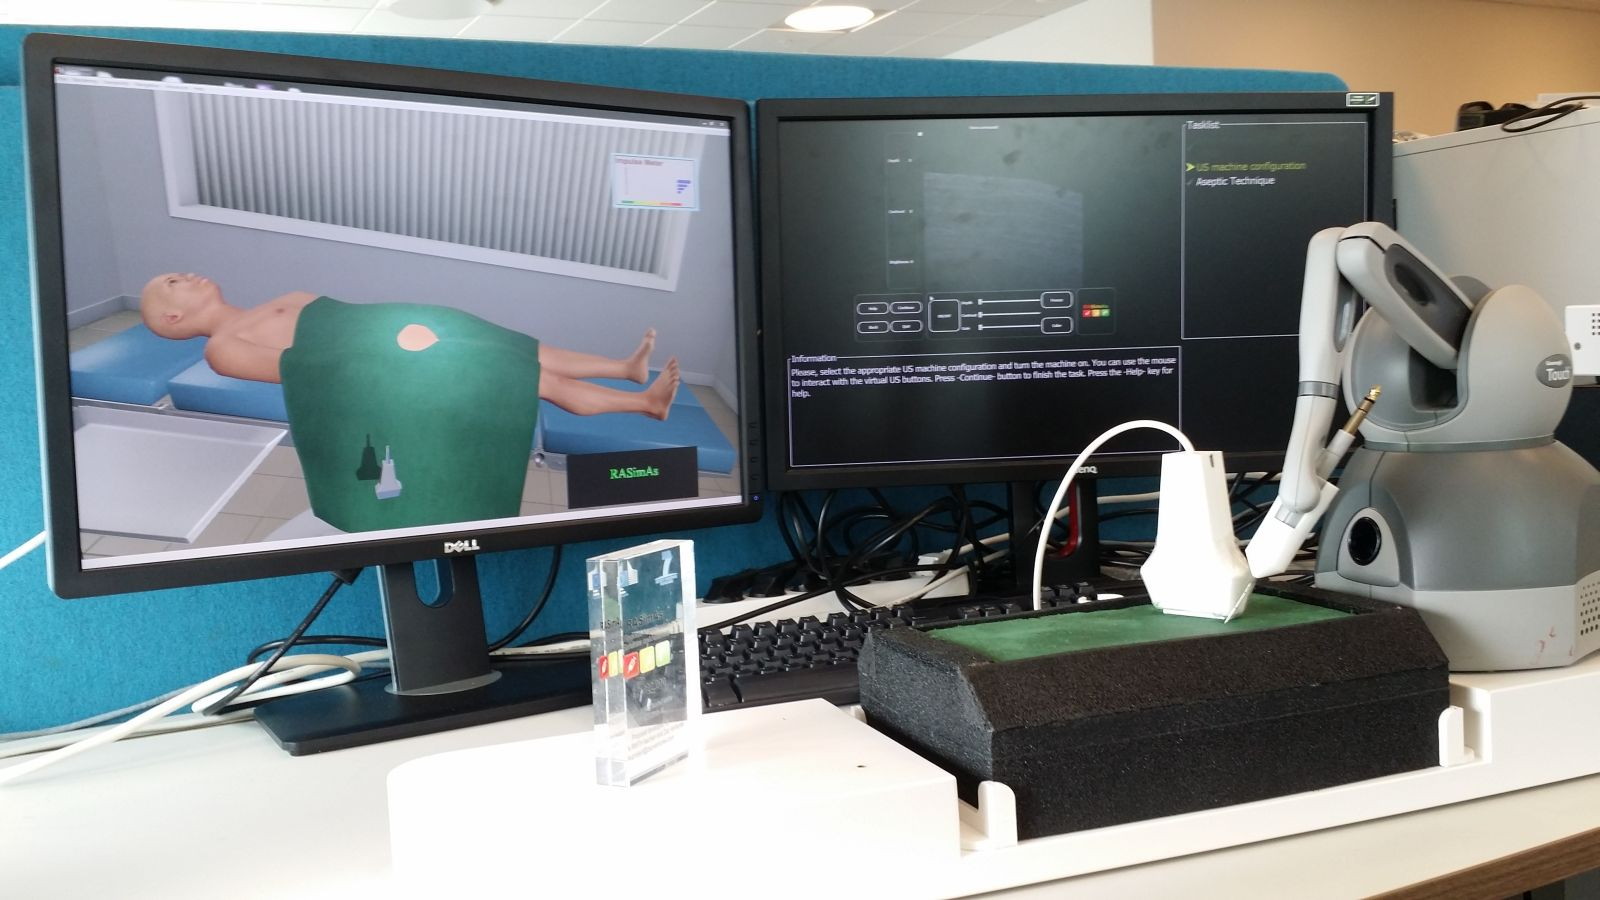
\includegraphics[width=1\textwidth]{IMG/sim3.jpg}
    \caption{RASim \label{subfig:introrasim}}
  \end{subfigure}%
  \begin{subfigure}[b]{0.5\linewidth}
    \centering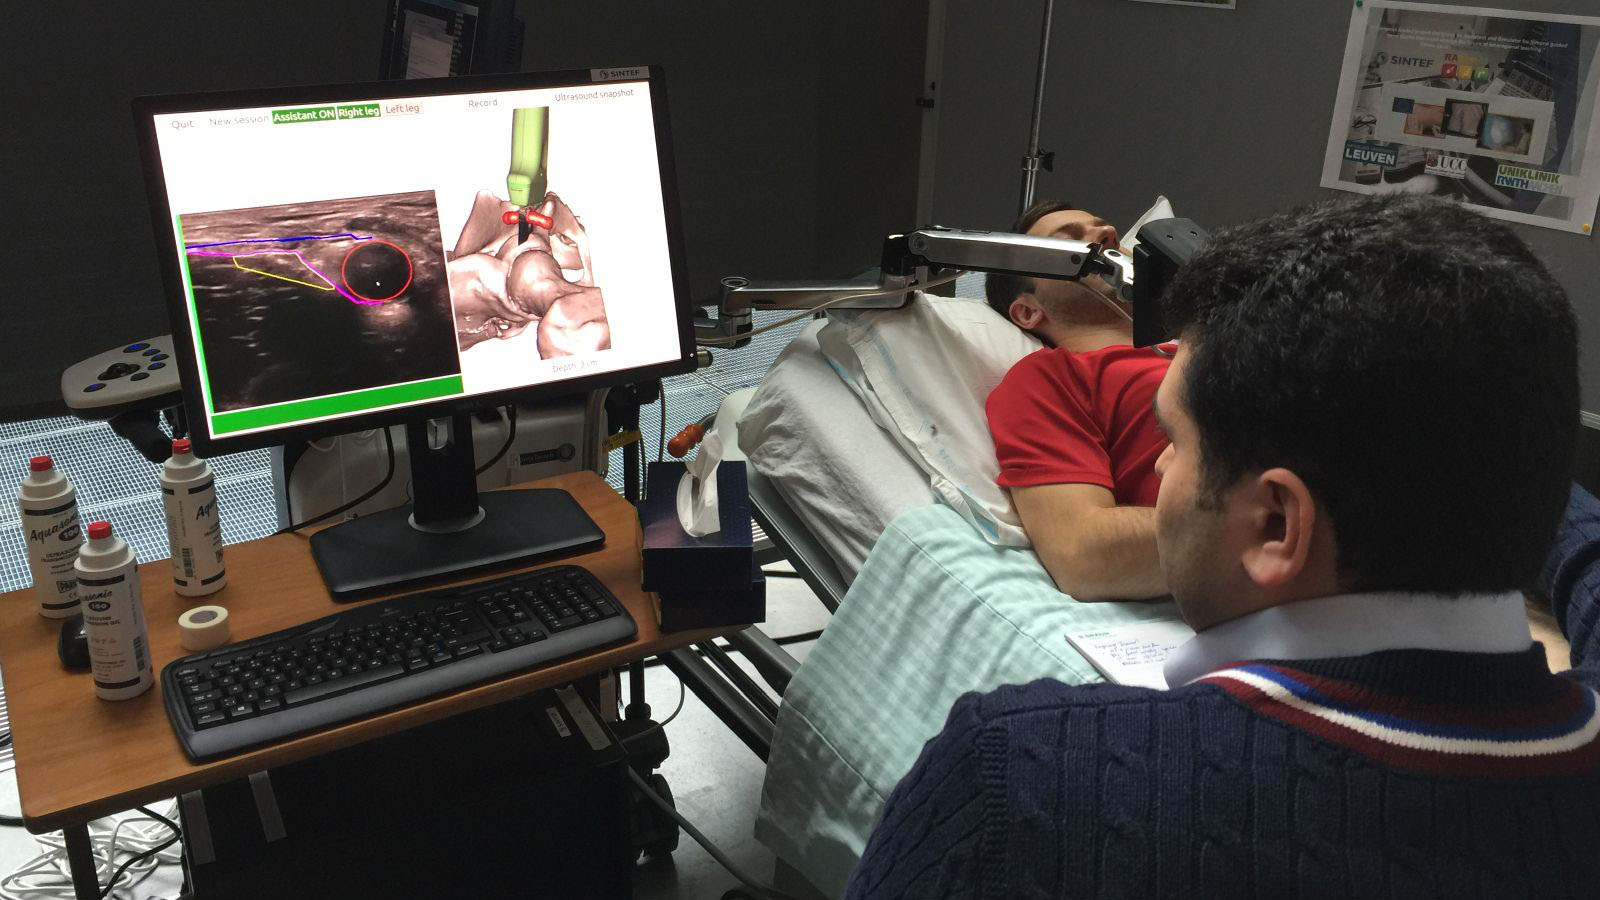
\includegraphics[width=1\textwidth]{IMG/raas.JPG}
    \caption{RAAs \label{subfig:introraas}}
  \end{subfigure}
  \caption{ Both RASimAs prototypes.}
\end{figure}



% %\todo{en pasado o presente?, pasado esta bien.}
% Esta tesis ha sido desarrollada dentro del contexto del proyecto \emph{RASimAs}, financiado por el 7º Programa del Marco de la Unión Europea. El objetivo principal es el desarrollo de herramientas que faciliten el entrenamiento y la práctica de la anestesia regional. Para cumplir con este objetivo se ha propuesto dos sistemas: un entrenador de realidad virtual llamado \emph{Regional Anaesthesia Simulator (RASim)} y un asistente en quirófano llamado \emph{Regional Anaesthesia Assistant (RAAs)}.

With the goal of facing a vast of anatomic variation, this project has proposed the development of a Virtual Physiological Human (VPH) database which it would be used in the \emph{RASim} simulator. An Integrated Toolkit for Generation of VPH Models (ITGVPH) has been developed for the generation of virtual patients based on patient-specific data. Additionally, it is required to transform the VPH models to the position required by the RA procedure. \emph{GMRV} group of the  \emph{Universidad Rey Juan Carlos} has been designated to lead this task.

% Con el objetivo de enfrentar a los médicos a la mayor cantidad de variabilidad anatómica posible, en este proyecto se ha propuesto desarrollar un entorno integrado de generación de pacientes virtuales, que permita crear una base de datos de modelos anatómicos que pueda ser utilizado por el simulador \emph{RASim}. Esta herramienta genera pacientes virtuales (VPH), a partir del registro de un modelo virtual con imágenes de pacientes reales. Además, es necesario transformar la postura del paciente generado a las diferentes posiciones requeridas por el procedimiento de anestesia regional. En concreto, esta tarea ha sido designada al grupo \emph{GMRV} de la \emph{Universidad Rey Juan Carlos}, estableciendo la motivación principal de esta tesis.

This thesis introduces a new technique that allows positioning the virtual patient models to the required position of the medical procedure. This new method works even if the virtual patient is incomplete or even if the mechanical model of the different tissues are not available. For this reason, it will be supervised by qualified physicians through a 3D UI. Therefore, the process must be interactive. To meet those requirements, a geometrically based approach have been followed. On the contrary, the physically based approach is not suitable because it needs a complete and proper model with the tissues' mechanic descriptions. Also, as they get accurate transformations, they required complex calculations that prevent interactive rates. Geometrical approaches provide plausible poses for training and educational purposes.

% A lo largo de este trabajo, se presenta una nueva técnica que permite transformar los modelos anatómicos de pacientes virtuales de su postura original a la posición necesaria por el procedimiento médico. Esto es posible aunque los modelos anatómicos se encuentren incompletos o falten sus descripciones mecánicas. Además, ya que el usuario supervisará la deformación que se aplicará al paciente virtual, el sistema debe tener tasas de refresco interactivas. Para cumplir con estos requisitos, se ha desarrollado una técnica geométrica basada en el cauce de la animación esqueletal, en lugar de utilizar un método basado en física debido a que estos últimos presentan una serie de problemas. En estos casos, se requiere caracterizar mecánicamente los tejidos que se van a simular los cuales no siempre se encuentran disponibles. Además, los métodos basados en modelos físicos se centran en conseguir deformaciones precisas, resultando en un alto grado de complejidad que impide conseguir tasas de refresco interactivas. Frente a los métodos basados en física, se ha optado por utilizar una técnica geométrica que proporciona soluciones plausibles que el usuario pueda interpretar como reales.

The proposed algorithm extends the classical skeletal animation pipeline to deal with character's internal tissues. From the skin and bones, our approach computes a displacement field from the bones’ movement, and uses it to transform the virtual tissues. Most of the complex tasks are computed during a pre-process stage, allowing to run the pose selection phase at interactive rates. It is fully automatic and it does not need users intervention.  Additionally, in order to refine the solutions, it was proposed an optimisation stage which uses a physically based approach in order to improve the volume conservation to achieve more appealing results. The figure \ref{fig:summaryarq} depicts the proposed animation pipeline stages. 



\begin{figure}[ht]
    \centering
    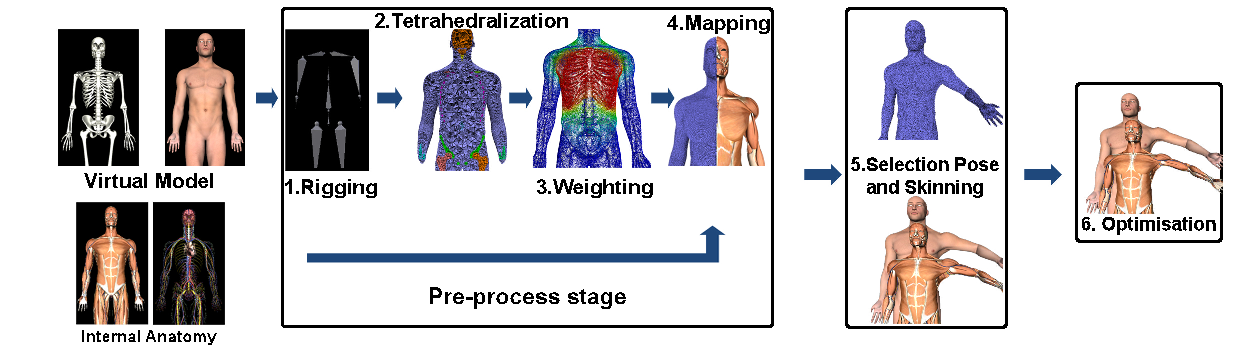
\includegraphics[width=0.95\textwidth]{IMG/summaryarq.pdf}
    \caption{Algorithm overview. First 4 steps represent the pre-process stage, Selection Pose and Skinning steps run at interactive rates and Optimisation phase is optional.}
    \label{fig:summaryarq}
\end{figure}

The following hypothesis has been formulated: "\emph{it is possible to create a geometrical algorithm which allows to transform the virtual patient pose with their internal tissues in order to use them in the context of medical training.}"  To validate it, two use cases have been developed.
% Partiendo de la piel y el tejido óseo del paciente virtual, se genera un campo de desplazamientos continuo en el interior del paciente virtual que se utiliza para transformar sus estructuras internas. Las operaciones más costosas se han delegado a un proceso previo que genera toda la información necesaria para que el usuario pueda seleccionar la postura del paciente virtual interactivamente. Además, se ha propuesto un refinamiento opcional basado en un método físico que intenta conservar el volumen del modelo anatómico. Con el objetivo de validar la hipótesis por la cual un algoritmo geométrico puede generar nuevas posturas de un paciente virtual junto con sus tejidos internos para ser utilizadas en el contexto del entrenamiento de un procedimiento médico, se han propuesto dos casos de uso. 


First, the proposed technique has been integrated into the ITGVPH, where it allows physicians to interactively animate a virtual patient. In this scenario, our algorithm works without complete models or mechanic properties. The pre-process stage must be performed once per model, but it automatically runs the complex steps avoiding the need of people with technical skills. Additionally, in order to prove the usefulness of those VPH in RA training, a courseware for the RASim simulator has been created. It provides a self-directed learning platform where trainees can rehearsal the procedure and improve their theoretical and non-cognitive skills. Courseware manages all simulation modules of RASim in order to develop training tasks. Unfortunately, haptic devices register manufacturing defects which made impossible to conduct a proper clinical trial of the simulator.

% En primer lugar, el algoritmo propuesto se ha integrado en el entorno de generación de pacientes virtuales, permitiendo animar y adaptar al profesional médico los modelos anatómicos generados por la suite. Se intenta demostrar que el algoritmo puede adaptar la postura de un modelo anatómico en un escenario donde no se dispone de modelos completos y no se dispongan de sus propiedades mecánicas. Además, con la finalidad de comprobar si los pacientes virtuales son útiles para  el entrenamiento del procedimiento de RA, se ha contribuido en la creación del módulo Courseware. Esta plataforma de aprendizaje donde el usuario podrá practicar y desarrollar sus habilidades no cognitivas, gestiona todos los componentes del simulador y se encarga de implementar las tareas de entrenamiento. Por problemas de precisión de los dispositivos hápticos, no se ha podido realizar una evaluación clínica del simulador. 
\begin{figure}[ht]
    \begin{subfigure}[b]{0.32\linewidth}
        \centering
        {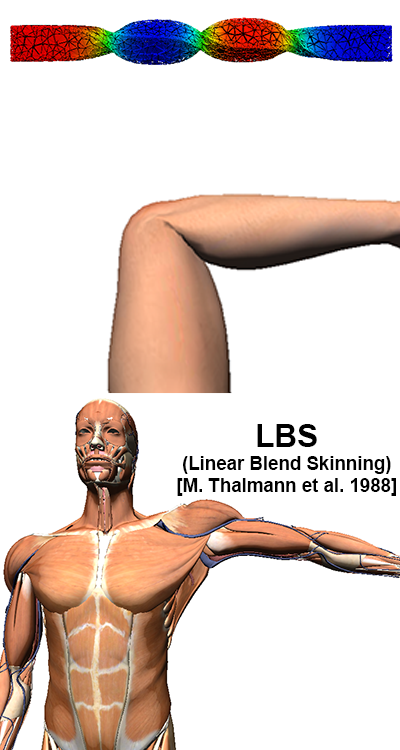
\includegraphics[width=\linewidth]{IMG/sLBS.png}}
        \caption{Bar model and \emph{ZygoteBody}$^{TM}$ transformed using linear blend skinning \label{subfig:sLBS}}
    \end{subfigure}
    \null\hfill
     \begin{subfigure}[b]{0.32\linewidth}
        \centering
        {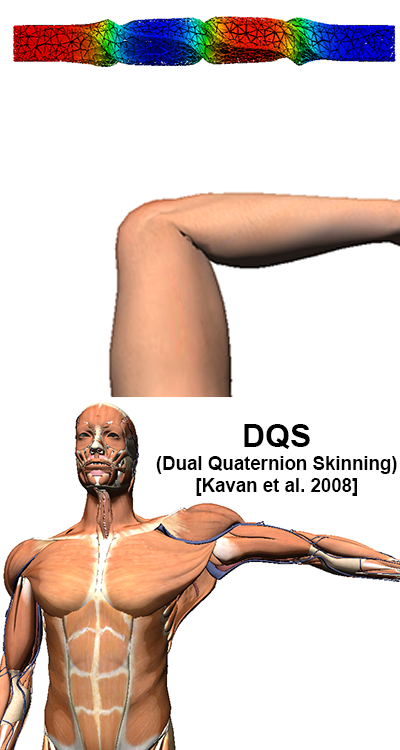
\includegraphics[width=\linewidth]{IMG/sDQS.png}}
        \caption{Bar model and \emph{ZygoteBody}$^{TM}$ transformed using dual quaternion skinning  \label{subfig:sDQS}}
    \end{subfigure}
    \null\hfill
     \begin{subfigure}[b]{0.32\linewidth}
        \centering
        {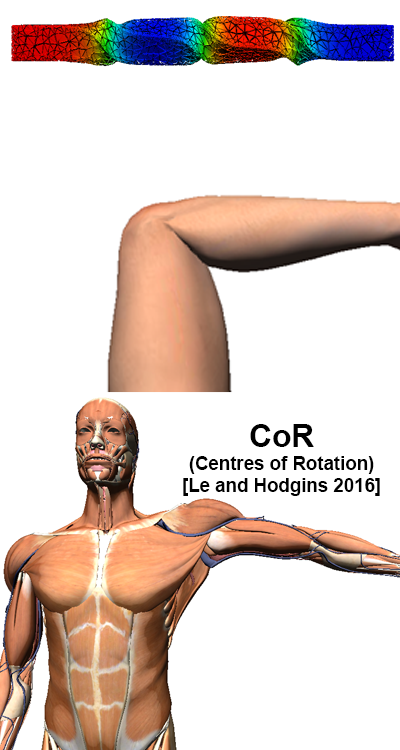
\includegraphics[width=\linewidth]{IMG/sCOR.png}}
        \caption{ Bar model and \emph{ZygoteBody}$^{TM}$ transformed using centres of rotation \label{subfig:sCOR}}
    \end{subfigure}
    \caption{\label{fig:compsummary} Some results obtained with three skinning techniques.}
   \end{figure}
Second, a projectional radiography simulator has been developed working closely with \emph{Dr. Franck P.Vidal}.   Projectional radiography (also called projection radiography, and X-ray radiography) is a very common medical imaging tool that supports clinicians in the diagnostic of certain diseases, infections, injuries (e.g.~bone fractures). Along the body, each specific location requires a correct patient positioning and X-ray machine configuration. Important aspects such as a convenience anatomic placement, collimation of the X-ray source, voltage of the X-ray tube, time of exposure, distance source to patient, and distance source to detector or film, must be dominated by radiographers in order to safely perform the procedure in a clinical environment. The simulator relies on the proposed technique and a real-time framework for the simulation of X-ray images provided by \emph{gVirtualXRay}\cite{sujar:hal}. Our method enables a user to pose interactively the virtual patient while \emph{gVirtualXRay} generates the corresponding X-ray image. Additionally, the proposed algorithm allows adding any external virtual patient model with the execution of the pre-process stage.  %The overall results  show that our tool is mostly realistic, useful and suitable in teaching and/or learning X-ray radiography.    

% En segundo lugar, se ha desarrollado un simulador de radiología diagnóstica gracias a la librería \emph{gVirtualXRay} en colaboración con \emph{Dr. Franck P.Vidal}. En este procedimiento, el médico debe posicionar al paciente y configurar la máquina de rayos X de manera que la región anatómica objetivo sea adecuadamente capturada. El algoritmo propuesto demuestra su capacidad para transformar la postura de un paciente virtual interactivamente, y así probar distintas proyecciones, mientras que la librería \emph{gVirtualXRay} permite  obtener imágenes de rayos X simultáneamente. Se ha realizado una encuesta a especialistas en radiología para comprobar su validez aparente y de contenido, donde se ha preguntado acerca de su opinión sobre el realismo y la utilidad del simulador. Los resultados obtenidos confirman su beneficio como herramienta adicional a las técnicas clásicas de aprendizaje.


Tests have been performed in order to evaluate the presented technique. In terms of performance, the preprocess take less than 7 minutes with the more complex virtual patient and it gets above 50 fps in the selection pose stage. For example, \emph{ZygoteBody}$^{TM}$ male model has close to $8 \times 10^5$ of vertices and $1.5\times 10^6$ of triangles; and produces an internal tetrahedral mesh which has close to $3.5\times 10^6$ of tetrahedrons and $8 \times 10^5$ of nodes.  Regarding the selected skinning technique, the two most used techniques are linear blending skinning (LBS) \cite{thalmann88} and dual quaternion skinning (DQS) \cite{Kavan2008}. They have been used, together with the new proposal which calculates optimal centres of rotation (COR) \cite{le2016real} for each vertex, by the algorithm to generate the results (see figure \ref{fig:compsummary}). 

In relation to ITGVPH, the proposed technique can work with incomplete models which come from this toolkit. For example, the figure \ref{fig:summarypatient} shows an incomplete model generated by ITGVPH with only the skin and bones, adapted by the proposed technique.
\begin{figure}[htbp]
    \centering
    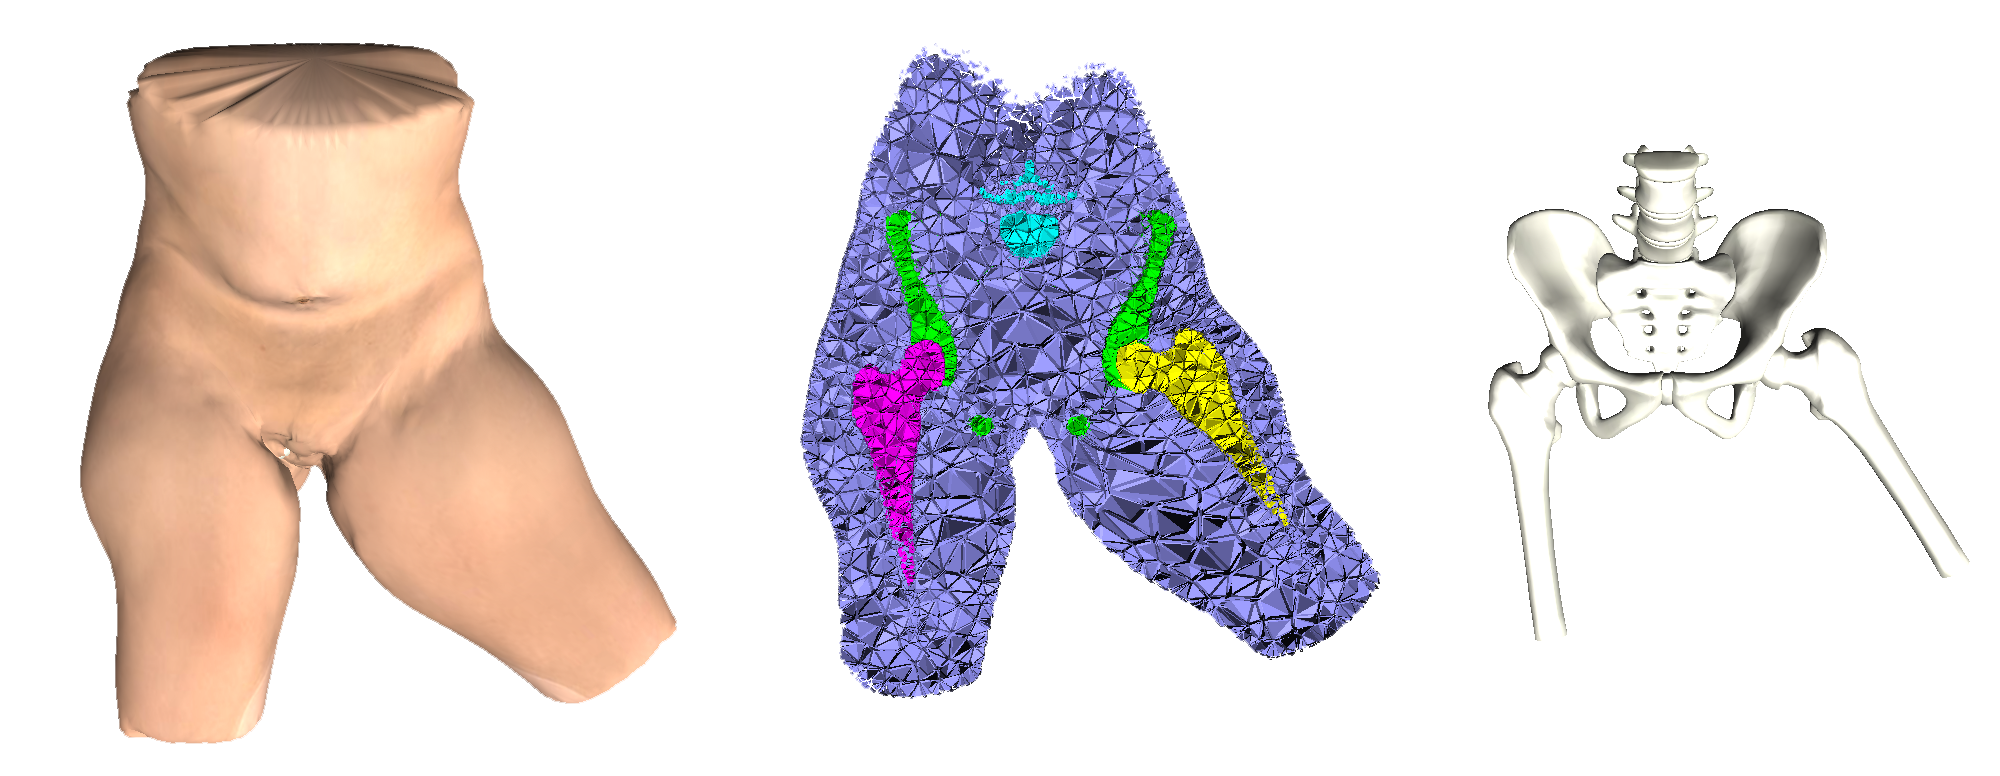
\includegraphics[width=0.95\textwidth]{IMG/spatient.png}
    \caption{Virtual patient model generated by ITGVPH and animated by the proposed technique.}
    \label{fig:summarypatient}
\end{figure}

Regarding the X-ray simulator (see fig. \ref{fig:summaryxray}), our algorithm together with \emph{gVirtualXRay} can run interactively above 25 fps and it could generate a variety of x-ray image from the input virtual patients. A promising face and content validation study have been conducted to gather  experts feedback. On one hand, the face validity performed shows that our tool is realistic in many ways.
The content validity performed shows both the usefulness and suitability of our tool in teaching and/or learning X-ray radiography. 



It is important to highlight that our geometric approachprovides a heuristic solution. Students do not need a specific patient model but a set of plausible virtual patients. This could be used for training and educational purposes.

\begin{figure}[htbp]
    \centering
    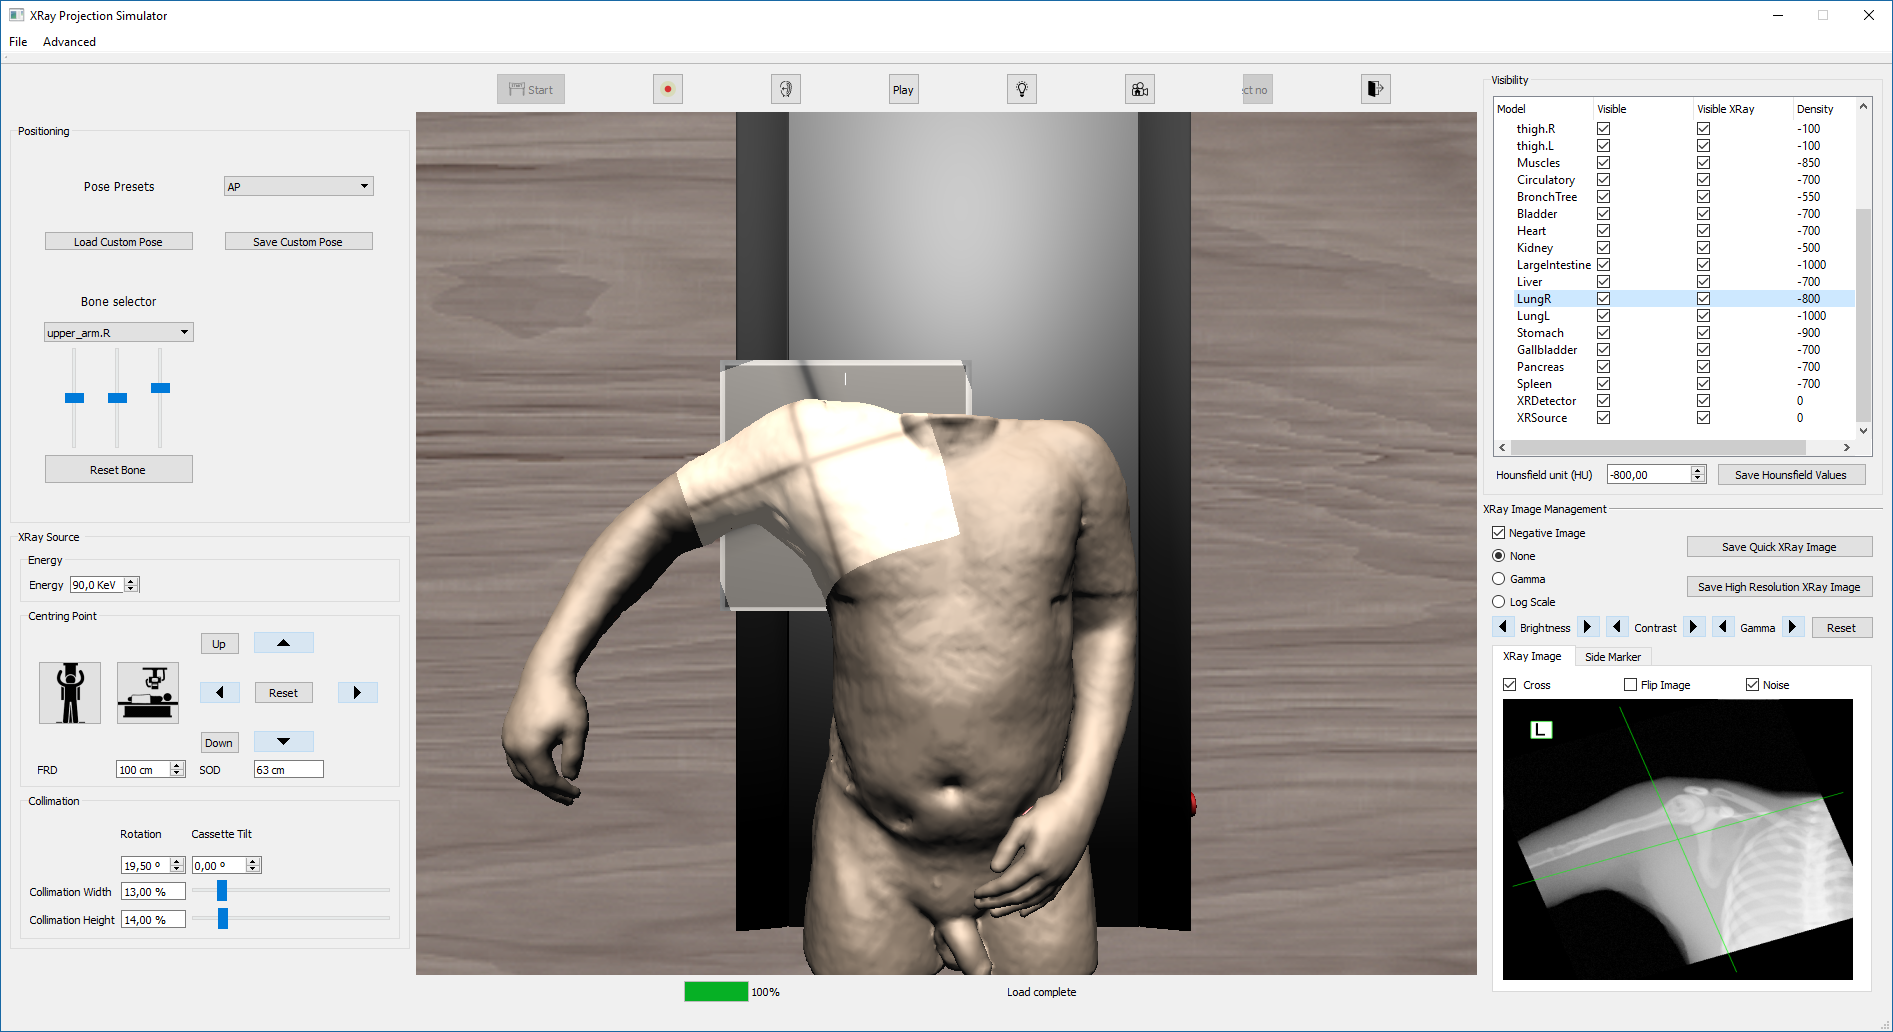
\includegraphics[width=0.95\textwidth]{IMG/suiteacher.png}
    \caption{UI of the X-ray simulator with the \emph{Segmented Inner Organs} \cite{VoxelMan}.}
    \label{fig:summaryxray}
\end{figure}

On one hand, it is worth to mention that the European Commission evaluated the \acs{RASimAs} project as \emph{Acceptable progress}. Although clinical trials were not conducted because of unexpected problems, they valued positively the \acs{RASim} prototype.

On the other hand, we present an interactive learning environment to teach radiography using real-time interactive X-ray simulation and to enhance the learning process. Face and content validity show both the usefulness and suitability of our tool.
\renewcommand{\figurename}{Figura}
